%%% PREAMBLE %%%

% Strict mode

\RequirePackage[l2tabu, orthodox]{nag} % Warn when using deprecated constructs

% Document class and packages

\documentclass[10pt,a4paper,parskip,fleqn]{scrartcl}
\usepackage[a4paper,vmargin={30mm},hmargin={30mm}]{geometry} % Page margins
\usepackage[ngerman]{babel} % New German hyphenation (multilingual support)
\usepackage[utf8x]{inputenc} % Unicode support
\usepackage{graphicx} % Graphics support
\usepackage{enumitem} % List spacing
\usepackage{nopageno} % No page numbers
\usepackage{chngpage} % Adjust page width
\usepackage{calc} % Calculations
\usepackage{color} % Colors
\usepackage{hyperref} % Hyperlinks

% Font configuration

\usepackage[sc]{mathpazo} % Use palatino font
\usepackage[T1]{fontenc} % Use correct font encoding
\usepackage[babel=true]{microtype} % Micro-typographic optimizations
\usepackage{setspace} % Line spacing
\addtokomafont{disposition}{\rmfamily} % Set palatino as heading font
\setstretch{1.3}
\setlist{nolistsep} % No spacing in lists


%%% TITLEPAGE %%%

\title{\Huge Coredump Rapperswil}
\subject{Sponsoring-Anfrage}


%%% MAIN DOCUMENT %%%

\begin{document}

\begin{titlepage}

	\maketitle

	\vspace{2cm}

	\begin{adjustwidth}{-\oddsidemargin-1in}{-\rightmargin-1in}
		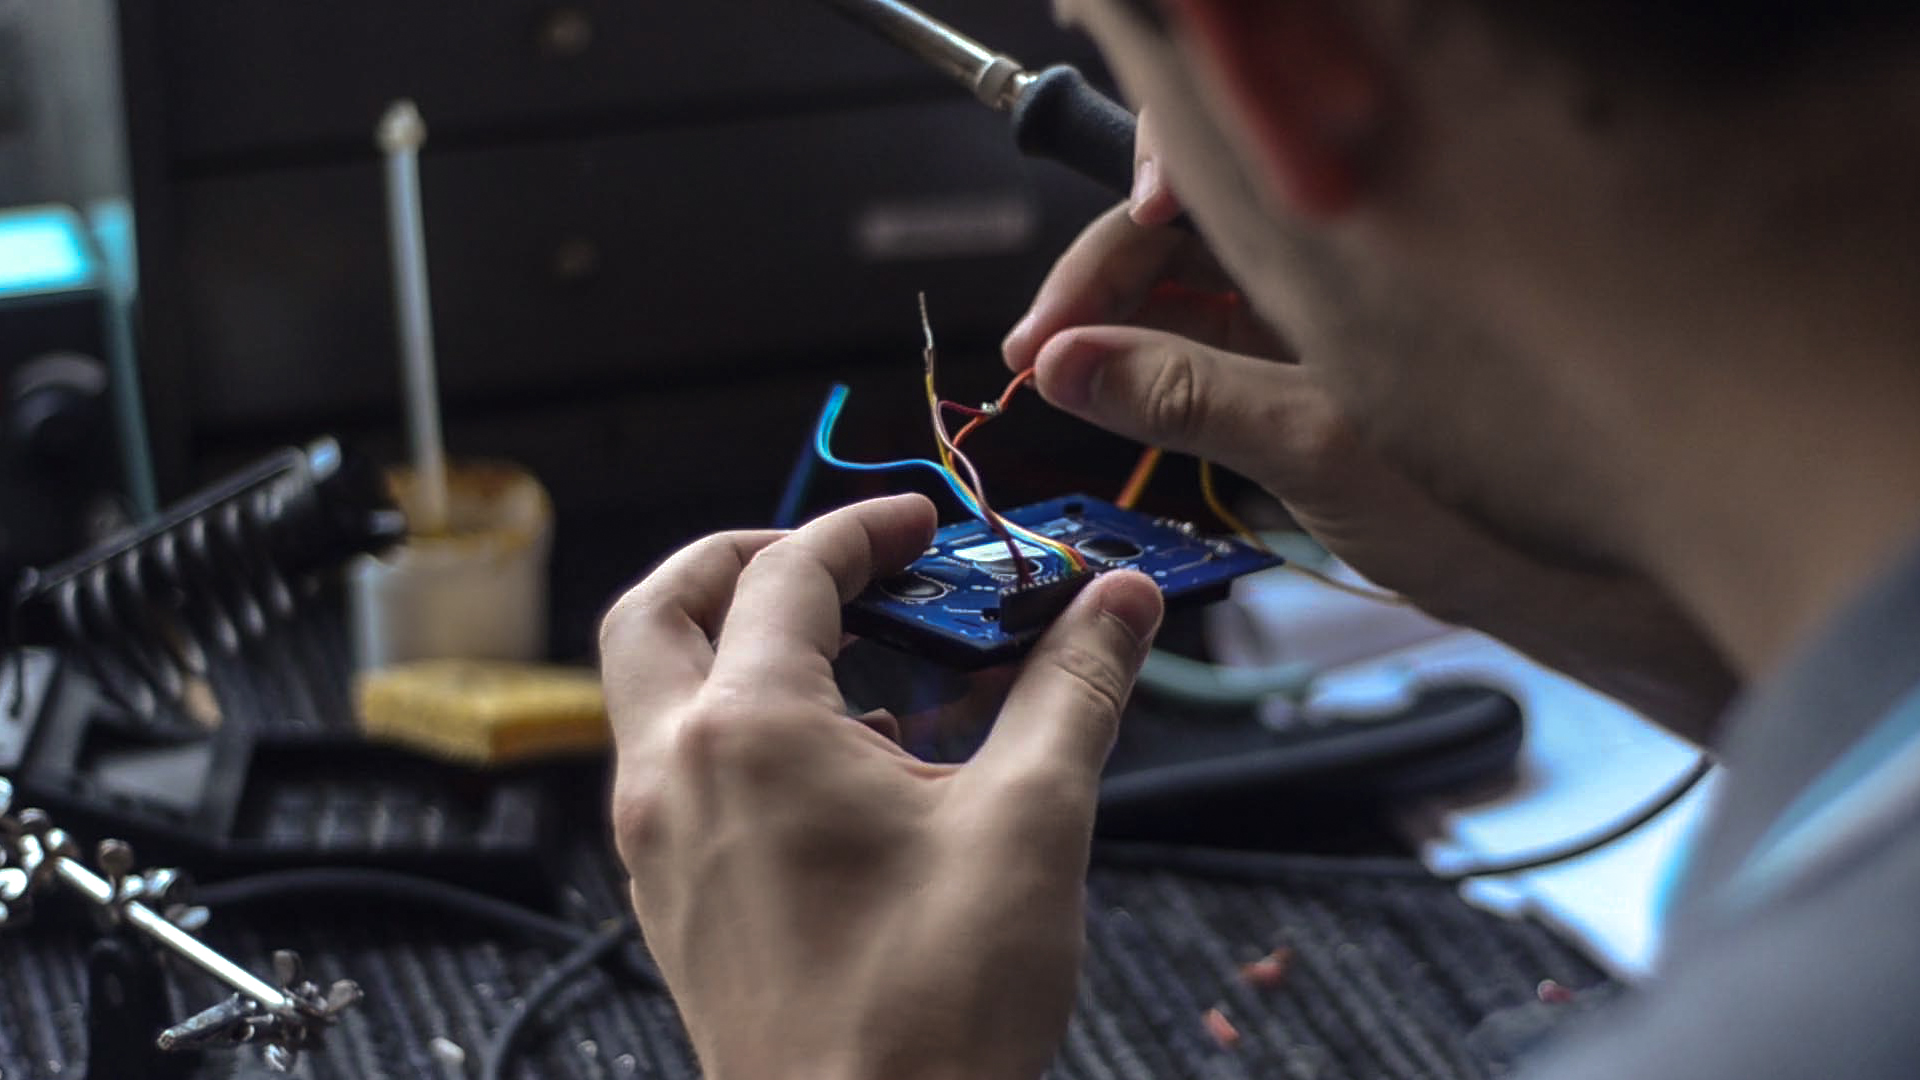
\includegraphics[width=\paperwidth]{soldering.jpg}

		\vspace{-12mm}

		\definecolor{light-gray}{gray}{0.85}
		\hfill {\scriptsize \color{light-gray} CC BY-NC-SA flickr.com/cbeas}
	\end{adjustwidth}

	\vfill

\end{titlepage}

\section{Über Uns}

Als erster Hackerspace\footnote{Mehr Informationen dazu gibt es auf
\url{http://hackerspaces.org/}} in Rapperswil-Jona bieten wir Computer- und
Technikbegeisterten seit August 2013 eine Plattform, in der sie ihr Wissen
weitergeben, austauschen und dazulernen können. Damit reihen wir uns in eine
weltweite Bewegung von tausenden von Hackerspaces, Makerspaces, FabLabs,
Techniklabors und ähnlichen Vereinen ein. Unser Angebot ist in der Region des
oberen Zürichsees bisher einzigartig.

Es geht dabei nicht um das <<Hacken von Computern>>, wie es in den Medien häufig
dargestellt wird, sondern gemäss der ursprünglichen Definition eines
Hackers\footnote{Mehr zur ursprünglichen Definition eines Hackers gibt es auf
Wikipedia: \url{https://de.wikipedia.org/wiki/Hacker}} um den kreativen Umgang
mit Technik und Wissen. Wir bieten Infrastruktur und KnowHow, um
nichtkommerzielle Projekte alleine oder in Kollaboration zu realisieren.

Unser zentral im Sonnenhof Rapperswil gelegener 50m²-Vereinsraum bietet aktuell
eine Elektronikwerkstatt mit Lötstation, Labornetzteil und Messgeräten, einen
3D-Drucker mit diversen Druckmaterialien, Arbeitsplätze für mitgebrachte
Laptops, WLAN mit Internetverbindung, ein Lager mit Elektronikbauteilen und
Entwicklungs-Kits, eine kleine Bibliothek mit Fachliteratur, einen Kühlschrank
und eine Mikrowelle für die Verpflegung vor Ort.

In unserem Hackerspace möchten wir einerseits die Möglichkeiten und das Umfeld
zur Umsetzung von interessanten technischen oder künstlerischen Projekten
anbieten, andererseits auch den Austausch von Wissen fördern. Dies kann
regelmässige Treffen, öffentliche Kurzvorträge oder auch Bildungsangebote und
Workshops für interessierte Aussenstehende (z.B. Ferienpass-Kurse für
Schulkinder) beinhalten.

\section{Projekte}

Damit Sie sich ein Bild unserer Aktivitäten machen können, nachfolgend drei
unserer aktuellen Projekte:

\textbf{Ferienpass im Computer- und Technikbereich}

Im November 2014 boten wir zum ersten Mal im Rahmen des Ferienpasses
Rapperswil-Jona\footnote{\url{Website: http://fepa-rj.ch/}} einen Löt- und einen
Programmierkurs für Kinder an. Diese -- wie auch wir selbst -- waren davon
begeistert: Wir erhielten 86 Anmeldungen und konnten davon aus Platzgründen
leider nur 16 berücksichtigen. Auch im Herbst 2015 und 2016 boten wir die Kurse
wieder an, mit sehr positivem Feedback. Wir freuen uns, auch in Zukunft
weiterhin Schulkinder aus Rapperswil-Jona mit Technik in Kontakt zu bringen und
dafür zu begeistern.

\newpage
\textbf{Wassertemperatursensoren Zürichsee}

Aktuell ist es für badefreudige Personen am Obersee schwierig, herauszufinden
wie warm oder kalt der See aktuell ist. Wir möchten deshalb in Kooperation mit
lokalen Vereinen sowie der Hochschule den Obersee (und später den Rest des
Zürichsees) mit einem Netzwerk aus solarbetriebenen Wassertemperatur-Sensoren
ausstatten und diese Messdaten öffentlich über Mobile Apps sowie auch über
Programmier-Schnittstellen zugänglich machen.

\textbf{3D-Druck}

Im Jahr 2015 durften wir unseren ersten 3D-Drucker in Betrieb nehmen,
erfolgreich finanziert über die Schweizer Crowdfunding-Plattform ``Wemakeit''.
Im Rahmen dieser Aktion haben wir unter anderem mit Hilfe eines Quadrokopters
einen 3D-Scan des Schlosses Rapperswil erstellt, diese Daten in Kooperation mit
der Hochschule für Technik HSR sowie dem Rapperswiler Start-Up ``Drei-De''
aufbereitet und ein druckfertiges Modell erzeugt.

\section{Finanzierung}

Bisher finanzieren wir uns primär über die Mitgliederbeiträge. Ein
Nichtverdiener-Mitglied bezahlt bei uns 10~CHF im Monat, ein Verdiener-Mitglied
30~CHF und ein Fördermitglied 50~CHF. Aktuell beläuft sich unsere
Mitglieder-Anzahl auf 25 Personen, die Meisten davon sind entweder Studenten an
der HSR oder haben bereits eine technische Ausbildung hinter sich. Daneben haben
wir einige privaten Gönner.

Unser Verein wächst stetig. Im Mai sind wir aus Platzmangel aus unserem
vorherigen 16m²-Vereinsraum in neue Räumlichkeiten im Sonnenhof umgezogen. Um
unser Angebot in Zukunft jedoch weiterhin ausbauen zu können, reichen die
Mitgliederbeiträge nicht ganz aus. Deshalb sind wir auf der Suche nach Gönnern
und Sponsoren, welche uns dabei unterstützen könnten.

Wir möchten folgende Sponsoring-Pakete vorschlagen:

\begin{itemize}
	\item Firmen-Sponsoring <<small>>: 80 CHF im Monat / 960 CHF im Jahr	
	\item Firmen-Sponsoring <<large>>: 120 CHF im Monat / 1440 CHF im Jahr	
\end{itemize}

Als Gegenleistung erhalten Sie als Sponsor folgende Möglichkeiten:

\begin{itemize}
	\item Einen Werbeplatz in unserem Vereinsraum: Ein A4-Blatt (<<small>>) bzw.
		ein A3-Blatt (<<large>>) auf dem Sie Ihre Firma vorstellen können oder
		schlicht Ihr Firmenlogo positionieren können. Das Blatt werden wir in
		unseren Räumlichkeiten an der Wand befestigen, wodurch sich Mitglieder und
		Besucher über Ihre Firma informieren können.
	\item Einen stets sichtbaren Link auf unserer Website. Zudem publizieren wir
		einen Blogpost auf unserer Website, in dem wir Sie als Sponsor vorstellen.
	\item Wir werden Sie als Unterstützer an jeder GV den Mitgliedern nochmals
		kurz vorstellen.
\end{itemize}

\section{Weitere Informationen}

Weitere Informationen zu uns und unserem Verein finden Sie auf unserer
Website:\\\url{https://www.coredump.ch/}.

Für Rückfragen können Sie den Vorstand unter \url{vorstand@lists.coredump.ch}
kontaktieren.

\end{document}
